\subsection{Future research direction}

\label{sec:intro}

\begin{frame}{Roadmap}
	\begin{block}{pLaTINUM context}
		\textit{Find the nearest sphere in the database according to a input composed of heterogeneous data}
	\end{block}
	
	We want to create an indirect method to localize a query within a set of geolocalized RGB-D spheres. The considered pipeline will be:
	\begin{itemize}
		\item \textbf<2>{Create a discriminative descriptor}
		\item Compute the representation of the spheres with our descriptor
		\item Compute the similarity of the query (also described by our descriptor) with the spheres representation
		\item Retrieve the closest sphere
	\end{itemize}
\end{frame}

\begin{frame}{Data representation}
	We first focus our work on creating a robust data representation. Research on state of the art shown that CNN are the best choice.
	
	\begin{block}{Encoder for data representation}
		\begin{figure}[c]
			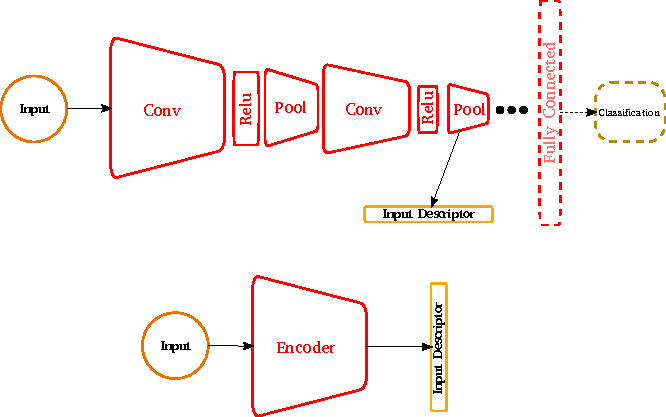
\includegraphics[width=0.75\linewidth]{vect/encodeur.pdf}					
		\end{figure}
	\end{block}
	
\end{frame}

\begin{frame}{Data representation}
	We begin with a pre-trained network and perform a fine tuning of its weights.
	\begin{block}{Encoder training for VBL task}
		\begin{figure}[c]
			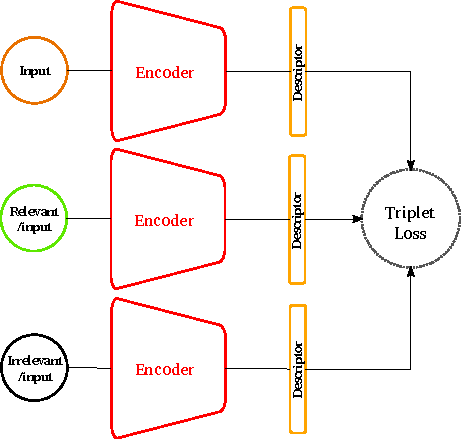
\includegraphics[width=0.5\linewidth]{vect/encoder_training.pdf}					
		\end{figure}
	\end{block}
\end{frame}

\begin{frame}{Multiple modalities}
	How to use more than one modality at the time?
	\vfill
	\begin{block}{Ideal Desired System specification}
		\centering
		\begin{tabular}{c | c}
			\textbf{Training data type} & \textbf{Testing data type} \\
			\hline
			RGB + Depth + Semantic & RGB +/or Depth +/or Semantic  \\
			+ Laser reflectance + ... &	+/or Laser reflectance +/or ... \\
		\end{tabular}
	\end{block}
	\vfill
	\begin{block}{What are we first trying to do}
		\centering
		\begin{tabular}{c | c}
			\textbf{Training data type} & \textbf{Testing data type} \\
			\hline
			RGB + (Depth or Laser reflectance)  & RGB  \\
		\end{tabular}
	\end{block}
\end{frame}